\documentclass[a4paper,12pt]{article}
\usepackage{graphicx}
\title{Cs 351 : Vending Machine }
\date{October 25, 2012}
\author{Khabbab Saleem}

\begin{document}
\maketitle


\section{Object Cube}

Clusters are made to make the object model a little bit more easier to understand.
each cluster and its function will be fined later on in section 2. 

\begin{center}
\begin{tabular}{l| p{10 cm}}
\hline
cluster & Objects\\
\hline
Key pad & makeDynamicKeyPad.js, keyPadActionListenerDollar.js\\
\hline
Product Holder & product.js, initializeProduct.js, makeDynamicTable.js, productTableActionListener.js\\
\hline
Dispenser  & productDispenser.js, reorderList.js
\end{tabular}
\end{center}

\section{Cluster Descriptions}

\subsection{Key pad}

Takes the input from the  and relays it to the D.O.M, where it can be accessed by any other cluster. This cluster is also responsible for returning the change. The conversion is done from the Euro to the Dollar via this as well. Machine will accept Euro but it will only use Dollar for the purchasing and returned change will also be in Dollars.

\subsection{Product Holder}
    Initially creates the table where the products are held by accessing the central table on the D.O.M. Displays the price, current quantity, and the  date, when the mouse is scrolled over said product. If the said item is expired or it has ran out, the alert will be sounded using the D.O.M. \\
\indent    	Communicates with the key pad, and the D.O.M when a product is selected to see is the current funds available on the machine are enough to dispense the product.
\subsection{Dispenser}
This is mainly ran from the Product Holder, when an item is clicked, when no error is throw by of alerts, the item is considered dispensed. All dispensed items are stacked on top of each other meaning when the item is clicked on the dispenser the item is fully dispensed.\\
\indent the reorder list is accessed by clicking the top right of the vending machine, it checks the main data structure in the product holder to see which of the item are below 5 (5 is current max value for the sake of testing). the reorder list is assembled based on the max value.   

\begin{figure}[ht!]
\centering
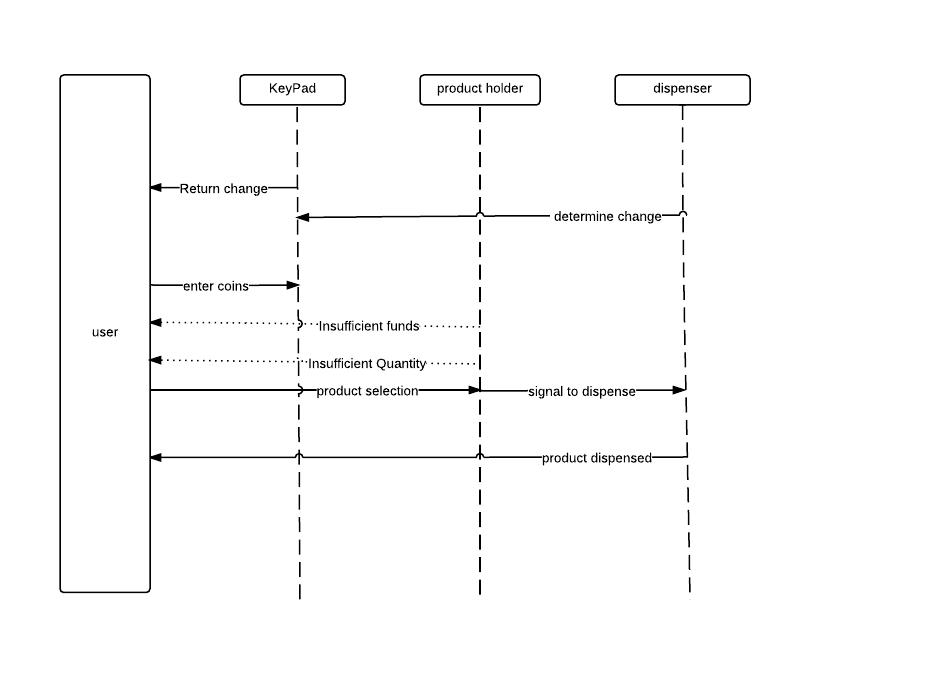
\includegraphics[scale=0.4]{interAction.jpeg}
\caption{interaction design}
\label{overflow}
\end{figure}





\begin{figure}[ht!]
\centering
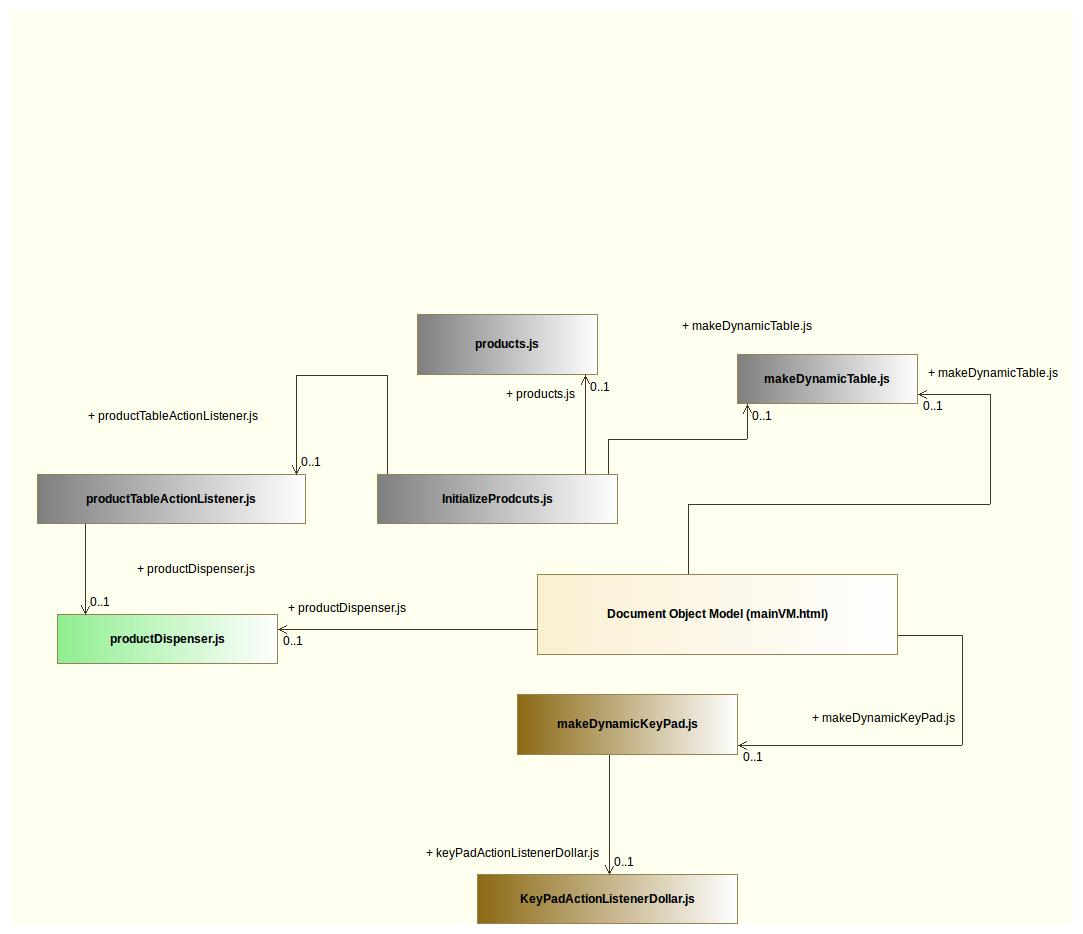
\includegraphics[scale=0.4]{ObjectModelvm.png}
\caption{Object Model}
\label{overflow}
\end{figure}

\end{document}